\chapter*{Appendices\label{part:appendices}}
\addcontentsline{toc}{chapter}{Appendices}

\renewcommand{\thesection}{\Alph{section}}
\section{Additional figures\label{sec:append.figures}}


\begin{figure}[H]
  \centering
  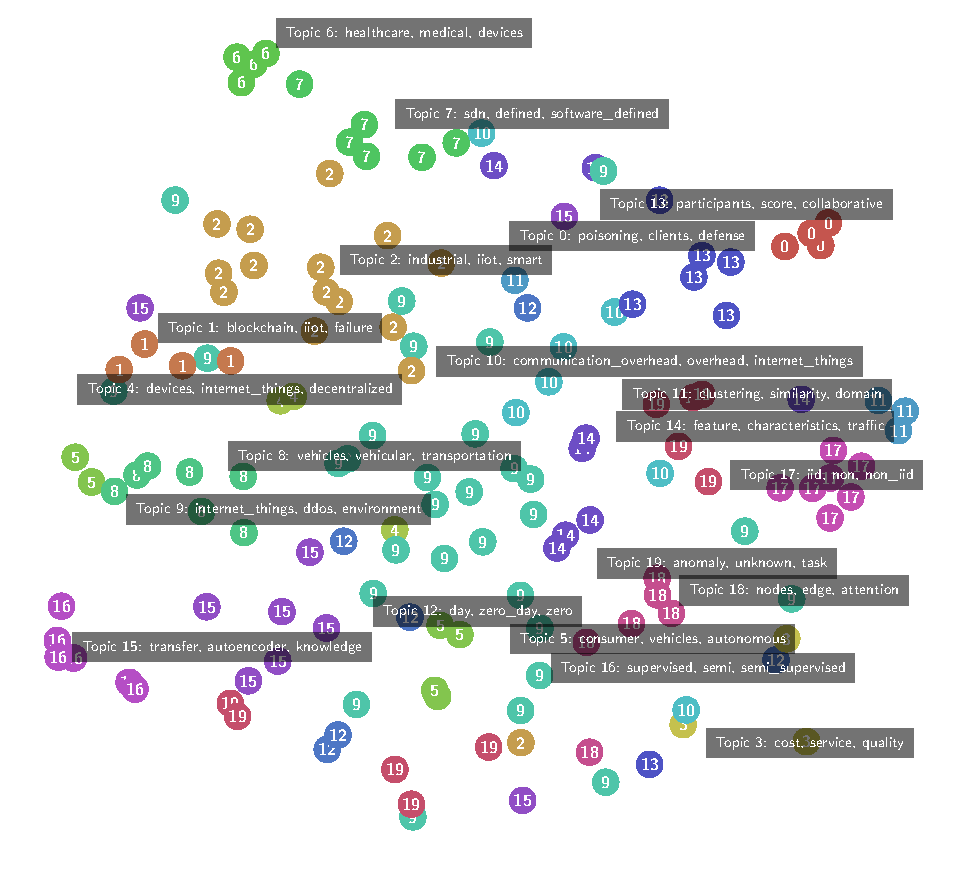
\includegraphics[width=\textwidth]{figures/topic_embedding.pdf}
  \caption{
    Topic embedding of the \gls{fids} literature using a \gls{nmf} model with 20 topics.
    Each point represents a paper, and each are labelled with the topic they are the most associated with.
    \label{fig:append.figure1}
  }
\end{figure}

% \begin{figure}
%   \centering
%   \begin{subfigure}
%     \centering
%     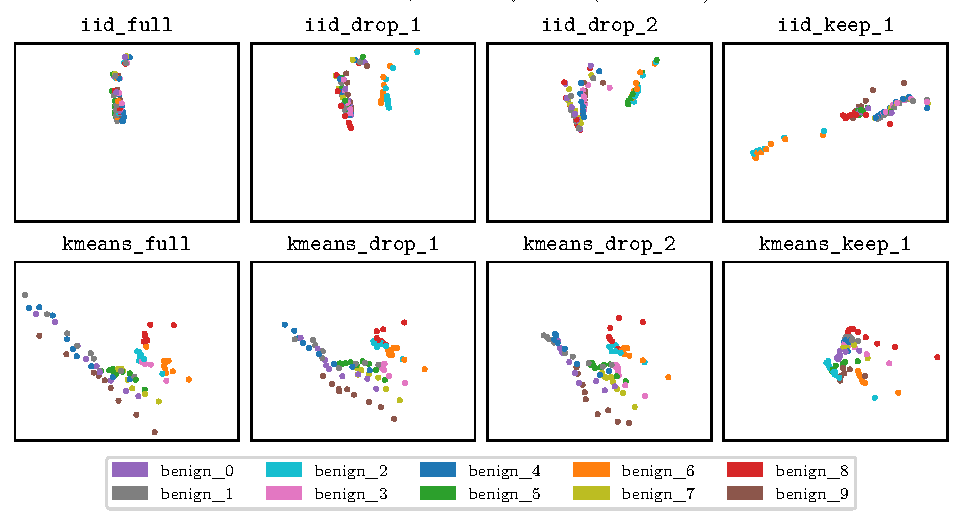
\includegraphics[width=\textwidth]{figures/cicids-grads-per-client.pdf}
%     \caption{CIC-CSE-CICIDS2018.}
%     \label{fig:append.grads-clients.cicids}
%   \end{subfigure}
%   \begin{subfigure}
%     \centering
%     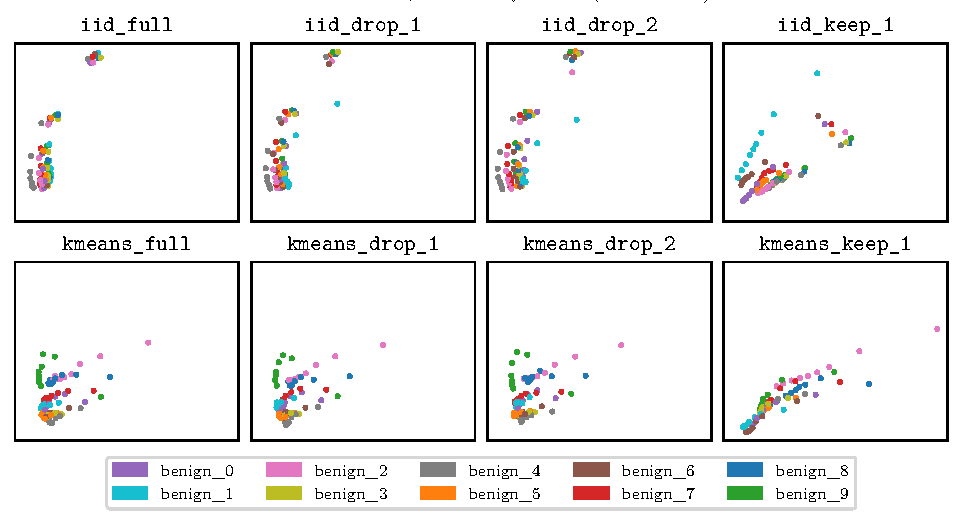
\includegraphics[width=\textwidth]{figures/nb15-grads-per-client.pdf}
%     \caption{UNSW-NB15.}
%     \label{fig:append.grads-clients.nb15}
%   \end{subfigure}
%   \caption{
%     2D projections of the gradients of the models trained on the CIC-CSE-CICIDS2018 and UNSW-NB15 datasets, with various partitioning schemes.

%     \label{fig:append.grads-clients}
%   }
% \end{figure}

\selectlanguage{french}
\selectlanguage{french}
\section{Résumé en français de la thèse\label{sec:french}}

La sécurisation des systèmes d'information se complexifie à mesure que ceux-ci gagnent en taille et en complexité. 
Parce que la sécurité par conception est bien souvent inapplicable, les différentes agences gouvernementales recommandent des mesures de sécurité complémentaires, telles que le déploiement de solutions de détection.
Les systèmes de détection d'intrusions (IDS en anglais) bénéficient grandement des dernières avances en apprentissage machine (ML), mais se heurtent aussi aux limitations de ces derniers.
En particulier, l'important coût humain et financier de la génération de données étiquetées pour entraîner des algorithmes d'apprentissage rend leur déploiement difficile pour les organisations.

Dans ce contexte, mettre en commun les données d'apprentissage permet d'améliorer la qualité de l'apprentissage, de réduire les biais dus aux distributions locales, tout en partageant de l'information sur des nouvelles classes d'attaques.
Malheureusement, les réglementations en vigueur (RGPD en tête), mais aussi la peur de la fuite d'information ou de propriété industrielle, rendent le partage de données impossible.

L'émergence de l'apprentissage fédéré (FL pour \emph{Federated Learning}) a relancé l'intérêt des communautés de détection d'intrusions pour les modèles collaboratifs.
Ce dernier permet d'entraîner un modèle unique sur des données réparties, sans pour autant qu'elles ne quittent leurs lieux de traitement respectifs.
Utilisé dans un contexte de détection d'intrusions, le FL permet d'étendre virtuellement la taille du jeu de données d'entraînement des participants.
Plus important encore, ce type d'algorithme permet aussi de propager des informations sur des caractéristiques apprises localement, en en faisant bénéficier d'autres organisations.
Cet apprentissage réparti promet enfin de palier certaines limitations classiques des algorithmes d'apprentissage, comme les biais de distribution.

Ainsi, l'application de l'apprentissage fédéré à la détection d'intrusions semble être une solution prometteuse pour améliorer les performances des IDS. Le nombre d'études publiées sur ce sujet corroborent cette hypothèse~\cite{lavaur_tnsm_2022,ismaila_ReviewApproachesFederated_2024}.
Néanmoins, cette approche pose de nouveaux défis, comme la gestion de l'hétérogénéité entre les participants ou la création de confiance entre ces derniers.
Plus généralement, \emph{Quelles sont les spécificités associées à l'application de l'apprentissage fédéré à la détection d'intrusions ? Le FL est-il une solution viable pour construire des IDS collaboratifs ?}


\subsubsection{Cas d'étude\label{sec:french.usecase}}

Parmi tous les cas d'usage possibles en détection d'intrusions, la détection d'intrusion au niveau réseau (NIDS) sur des systèmes d'information orientés IT se trouve particulièrement représenté.
Cela a un intérêt pratique, notamment pour la disponibilité d'algorithmes déjà implémentés et de jeux de données appropriés.
L'intérêt en terme d'évaluation est évident, puisque cela rend les approches comparables, notamment en termes de performance. 

De plus, ce cas d'étude représente un cas d'application réaliste pour des systèmes de détection d'intrusions fédérés, où les participants à ce type de systèmes sont des organisations en charge de la surveillance d'un système d'information.
À titre d'exemple, un NIDS fédéré pourrait être déployé entre les Centre Opérationnels de Sécurité (SOC) de plusieurs entreprises, qui auraient intérêt à partager des informations sur les attaques qu'ils ont détectées, sans pour autant partager les données brutes.


\subsubsection{Questions de recherche\label{sec:french.questions}}

La problématique traitée par cette thèse peut être résumée par la question suivante : \emph{L'apprentissage fédéré peut-il fournir un cadre fiable de partage de connaissances pour améliorer de manière collaborative les mécanismes de détection d'intrusion ?}

\begin{questions}
  \item Qu'y a-t-il de spécifique à l'application de l'apprentissage fédéré aux IDS ?
  \item L'apprentissage fédéré peut-il être utilisé pour entraîner des IDS à partir de sources de données hétérogènes ?
  \item Comment l'apprentissage fédéré gère-t-il les contributions malveillantes dans un IDS fédéré ?
  \item Comment évaluer et garantir la fiabilité des contributions des autres participants ?
\end{questions}


\subsection{Résumé des contributions\label{sec:french.summary}}

Dans le chapitre \nameref{chap:intro} de ce manuscrit, après avoir présenté le contexte et les motivations de ce travail, nous formulons notre objectif de recherche sous la forme de la question de recherche énoncée ci-dessus.
Nous déclinons cet objectif en quatre questions de recherche (\Cref{rq:intro.fids,rq:intro.heterogeneity,rq:intro.malicious,rq:intro.trust}) et structurons le reste de ce manuscrit autour de ces questions.  
La première partie de ce manuscrit, \Cref{part:fids}, est exploratoire et vise à comprendre les caractéristiques fondamentales des Systèmes de Détection d'Intrusions Fédérés (FIDS).  
Nous commençons par fournir les connaissances de base sur les systèmes de détection d'intrusions et l'apprentissage fédéré dans \Cref{chap:background}, avant de passer en revue l'état de l'art des IDS collaboratifs (CIDS) et du FL dans \Cref{chap:sota}, abordant ainsi la question \Cref{rq:intro.fids}.  
Cette première partie se termine par l'illustration du potentiel des FIDS à travers une application pratique dans \Cref{chap:application}, mettant en lumière les défis associés aux questions \Cref{rq:intro.heterogeneity,rq:intro.malicious} : l'hétérogénéité des données et la présence de participants malveillants.  
La deuxième partie de ce manuscrit, \Cref{part:contribs}, se concentre sur la résolution de certaines des limitations identifiées des FIDS, afin de répondre aux questions \Cref{rq:intro.heterogeneity,rq:intro.malicious,rq:intro.trust}.  
Nous répondons ici à ces questions de recherche, en renvoyant aux chapitres correspondants.


\subsubsection{Réponses aux questions de recherche\label{sec:conclusion.contribs.answers}}

\begin{itemize}[listparindent=\parindent,itemsep=.6\baselineskip]

  \item \Cref{rq:intro.fids} : \emph{Qu'y a-t-il de spécifique à l'application de l'apprentissage fédéré aux IDS ?}

  En introduisant les concepts préliminaires nécessaires à cette thèse dans \Cref{chap:background}, nous énumérons les défis des CIDS qui motivent l'exploration du FL.  
  Cela ne suffit pas à répondre à la question, nous réalisons donc une revue complète de l'état de l'art dans \Cref{chap:sota}, où nous proposons une taxonomie qui décrit les FIDS selon cinq axes : \emph{données}, \emph{opération locale}, \emph{paramètres de fédération}, \emph{agrégation}, et \emph{évaluation}.  
  Cela met en évidence la première spécificité des FIDS, puisque deux de nos cinq critères couvrent la plupart des taxonomies existantes du FL : \emph{paramètres de fédération} et \emph{agrégation}.  

  Nous discutons dans le même chapitre d'autres aspects critiques de la détection d'intrusion, en insistant sur l'importance de l'explicabilité, de la personnalisation et de la robustesse face aux attaques dans ce contexte.  
  De plus, les types spécifiques de distributions et de partitions de données rencontrés dans les IDS sont uniques à ce domaine, comme le chevauchement des classes d'attaques observé dans \Cref{chap:assessment}.  
  Enfin, le manque de jeux de données et la grande diversité des cas d'usage des IDS rendent difficile la généralisation des résultats de la recherche en FL dans ce domaine.

  \item \Cref{rq:intro.heterogeneity} : \emph{L'apprentissage fédéré peut-il être utilisé pour entraîner des IDS à partir de sources de données hétérogènes ?}

  Observée à la fois dans la littérature sur le FL et les FIDS (\cf \Cref{chap:sota}), l'hétérogénéité des données représente un défi majeur pour les déploiements réels du FL.  
  Nous illustrons ce problème dans \Cref{chap:application}, où nous mettons en avant à la fois les avantages de l'hétérogénéité des données (\eg, une meilleure généralisation et un partage de connaissances amélioré) et les défis qu'elle pose, notamment en termes de convergence et de performance.  
  \Cref{chap:assessment} souligne un autre problème lié à l'hétérogénéité des données : lorsque les participants sont trop différents, il devient plus difficile d'identifier les contributions malveillantes.

  Nous proposons dans \Cref{chap:radar} une approche novatrice pour résoudre ce problème, \texttt{RADAR}, qui repose sur trois composantes :  
  \begin{enumerate*}[(i)]
    \item un schéma de \emph{cross-evaluation} (ou évaluation croisée) qui modifie l'algorithme classique du FL pour intégrer des retours d'évaluation ;  
    \item un algorithme de \emph{clustering} qui regroupe les participants en fonction des similitudes de leurs retours, offrant une vue plus subjective des différences entre participants ; et  
    \item un système de \emph{réputation} qui analyse les retours au fil du temps pour pondérer le processus d'agrégation en conséquence.  
  \end{enumerate*}  
  Cependant, en raison du manque de jeux de données appropriés pour les IDS répartis, notre évaluation reste limitée.  
  Nous proposons donc dans \Cref{chap:topologies} une approche non conventionnelle pour résoudre ce problème, en utilisant la composition de topologies basées sur des contraintes pour générer des jeux de données synthétiques imitant les caractéristiques des organisations indépendantes.  
  Par conséquent, bien que nous disposions d'éléments de preuve que le FL pourrait être utilisé pour fédérer des IDS à partir de sources de données hétérogènes, cela reste une direction de recherche majeure.

  \item \Cref{rq:intro.malicious} : \emph{Comment l'apprentissage fédéré gère-t-il les contributions malveillantes dans un IDS fédéré ?}

  Les participants malveillants représentent une menace majeure pour les systèmes collaboratifs.  
  Le FL n'échappe pas à cette règle, et nous illustrons dans \Cref{chap:application} comment l'absence de contrôle sur les contributions des participants constitue effectivement un problème majeur.  
  Pour mieux comprendre cette problématique, nous réalisons une analyse systématique de l'impact des attaques par inversion de labels contre un FIDS dans \Cref{chap:assessment}, et construisons un cadre d'évaluation pour faciliter ce processus.  
  Les attaques par inversion de labels sont particulièrement intéressantes, car elles sont faciles à mettre en œuvre et peuvent être appliquées à tout modèle de menace.  
  Nos résultats montrent que l'impact de ces attaques peut être assez important, mais que la construction inhérente du FL permet également d'atténuer partiellement leur effet, jusqu'à un certain seuil.  
  Avec \Cref{chap:radar}, nous introduisons une approche novatrice pour détecter les participants malveillants, y compris les grands groupes d'attaquants en collusion.  
  Cependant, nos expériences doivent être étendues pour généraliser nos conclusions.

  \item \Cref{rq:intro.trust} : \emph{Comment évaluer et garantir la fiabilité des contributions des autres participants ?}

  Même sans intention malveillante, les mises à jour de modèles téléchargées peuvent avoir un impact négatif sur le modèle global.  
  Cela peut s'expliquer par l'hétérogénéité (voir \Cref{rq:intro.heterogeneity,chap:application}), mais aussi par la qualité des données d'entraînement.  
  \texttt{RADAR} (\Cref{chap:radar}) constitue un premier pas vers la résolution de ce problème, car il offre des garanties sur la qualité des contributions des participants, basées sur des métriques d'évaluation.  
  En fait, du point de vue de notre agrégateur, savoir si un participant est malveillant ou non est sans importance : les retours recueillis évaluent la qualité du modèle, pas les intentions des participants.  
  Surtout, \texttt{RADAR} est, à notre connaissance, la seule approche de FL tenant compte de la réputation qui exploite les retours réels des participants.  
  Cela représente un changement majeur dans la manière d'évaluer la fiabilité des contributions des participants, en relâchant l'hypothèse selon laquelle les participants ne peuvent télécharger que des mises à jour de modèles.

\end{itemize}


\subsection{Travaux futurs et perspectives d'évaluation\label{sec:french.future}}

Cette thèse a ouvert la voie à l'exploration des systèmes de détection d'intrusions collaboratifs basés sur l'apprentissage fédéré (FL), en abordant les défis liés à la sécurité et à l'efficacité de ces systèmes.
Certaines limitations demeurent néanmoins, notamment en ce qui concerne l'extension des études d'évaluation et la génération de jeux de données adaptés à des scénarios distribués.
La conclusion de ce manuscrit (\Cref{chap:conclusion}) résume les contributions de cette thèse, avant de décrire comment les travaux futurs pourraient résoudre leurs limitations et améliorer l'état de l'art des FIDS dans \Cref{sec:conclusion.future}.
Cette dernière partie résume ces pistes de recherche, ainsi que les perspectives plus larges à même de guider les travaux sur les CIDS, au-delà des contributions actuelles.

Dans le cadre de la poursuite des travaux présentés dans ce manuscrit, les améliorations porteront d'abord sur l'extension des études d'évaluation des attaques par empoisonnement de modèles fédérés, au-delà des simples attaques par inversion de labels déjà examinées dans cette thèse.
Il sera nécessaire de tester différentes méthodes d'empoisonnement de modèle et d'intégrer de nouveaux jeux de données pour obtenir une vue d'ensemble plus complète de la fiabilité des CIDS face à de telles menaces.
Une deuxième piste repose sur l'amélioration du passage à l'échelle de \texttt{RADAR} en développant des mécanismes décentralisés via des protocoles pair-à-pair, ce qui permettrait de gérer un plus grand nombre de participants sans compromettre la performance ou la confidentialité des échanges.
Enfin, la génération de données réparties réellement indépendantes représente un autre chantier crucial, avec l'objectif ici de faire passer \verb|FedITN_gen| de la simple génération de topologies à des scénarios complets, pour valider les approches dans des environnements plus proches de la réalité.

Le manuscrit détaille aussi des perspectives à long terme, incluant plusieurs axes de recherche pour faire évoluer les CIDS.
Tout d’abord, les stratégies d’agrégation des modèles fédérées peuvent bénéficier des progrès récents en matière de confidentialité différentielle (\emph{differential privacy}) et de robustesse face aux attaques.
Ensuite, l’intégration des systèmes décentralisés pose de nouveaux défis en termes de confiance entre les participants et d’interopérabilité des modèles, qui devront être résolus pour déployer ces systèmes à grande échelle.
L’évaluation des CIDS elle-même doit par ailleurs être approfondie, notamment en créant de nouveaux benchmarks et en établissant des méthodologies robustes pour garantir la reproductibilité des résultats dans des environnements distribués.
Enfin, l’évolution du cadre réglementaire, avec des lois et directives telles que le RGPD et l'AI Act, soulève également des questions sur la conformité des approches fédérées, notamment en matière de partage sécurisé de connaissances et de respect de la confidentialité des données locales.
Ces recherches, à la croisée de la cybersécurité et de la réglementation, façonneront l'avenir des systèmes collaboratifs pour la cybersécurité.